\documentclass[12pt,letterpaper]{article}
\usepackage{fullpage}
\usepackage[top=2cm, bottom=4.5cm, left=2.5cm, right=2.5cm]{geometry}
\usepackage{amsmath,amsthm,amsfonts,amssymb,amscd}
\usepackage{algorithm}
\usepackage{algorithmic}
\usepackage{lastpage}
\usepackage{enumerate}
\usepackage{fancyhdr}
\usepackage{mathrsfs}
\usepackage{xcolor}
\usepackage{graphicx}
\usepackage{listings}
\usepackage{hyperref}
\usepackage{indentfirst}
\usepackage{setspace}
\doublespacing
\renewcommand{\thesubsection}{\thesection.\alph{subsection}}
\hypersetup{%
  colorlinks=true,
  linkcolor=blue,
  linkbordercolor={0 0 1}
}
 
\renewcommand\lstlistingname{Algorithm}
\renewcommand\lstlistlistingname{Algorithms}
\def\lstlistingautorefname{Alg.}

\lstdefinestyle{Python}{
    language        = Python,
    frame           = lines, 
    basicstyle      = \footnotesize,
    keywordstyle    = \color{blue},
    stringstyle     = \color{green},
    commentstyle    = \color{red}\ttfamily
}

\setlength{\parindent}{0.0in}
\setlength{\parskip}{0.05in}

% Edit these as appropriate
\newcommand\course{Linear Algebra}
\newcommand\NetIDa{Brian Hotopp}           % <-- NetID of person #1

\pagestyle{fancyplain}
\setlength{\parindent}{20pt}
\headheight 35pt
\lhead{\NetIDa}
\lhead{\NetIDa}                 % <-- Comment this line out for problem sets (make sure you are person #1)
\chead{\textbf{\Large Final Project}}
\rhead{\course}
\lfoot{}
\cfoot{}
\rfoot{\small\thepage}
\headsep 1.5em
\begin{document}
\section{Word Embeddings}
For my final project I chose to apply principal component analysis to word embeddings.
Word embeddings allow the representation of words as vectors, where words with similar meanings have similar vector representations. One naive algorithm to embed words into a vector space would be to gather the set of all words in the input dataset, and then collect for each word the frequencies of its neighbors across all its occurrences (within some fixed window). For example to embed the word "math" using this algorithm, we would initialize the embedding of "math" as an n-dimensional vector where n is the number of unique words in the dataset. We would then look at each occurrence of "math" in the input dataset, and for the words within some distance of "math," we would increment their corresponding count in the embedding. When we finish this process, the resulting vector captures which words in the corpus "math" occurs most frequently around.

In practice this approach is not commonly used, because there are many unique words in large corpora, and therefore if we were to use this technique the embeddings generated would be extremely high-dimensional. Instead, a popular approach for generating word embeddings is to use Word2Vec, a technique published by Google in 2013. Word2Vec that uses a shallow neural network to embed words into a vector space, usually of some dimension between 100 and 1000. I used the \texttt{gensim} library in python to generate word embeddings of dimension 100 for my analysis.
\cite{lamport94} is a set of macros built atop
\section{Dataset}
For my dataset I chose to use the Brown Corpus, which is a large compilation of American English, containing roughly one million words. It was compiled at Brown university in 1961, and it contains 500 samples across many different genres. The \texttt{nltk} python package provides a simple interface for the Brown Corpus, which I used to generate my word embeddings.
\section{PCA And Results}
I implemented PCA so I could reduce the dimensionality of the resulting word embeddings from dimension 100 to dimension 2. This allows the word embeddings to be visualized in 2d plots. Here are some example words for which I found the top 10 nearest neighbors in the 2d vector space using cosine similarity, and used my implementation of PCA to reduce the set of 11 100-dimensional vectors to a set of 11 2-dimensional vectors. I then used the \texttt{matplotlib} python library to make scatter plots.
\begin{figure}[H]
\begin{center}
  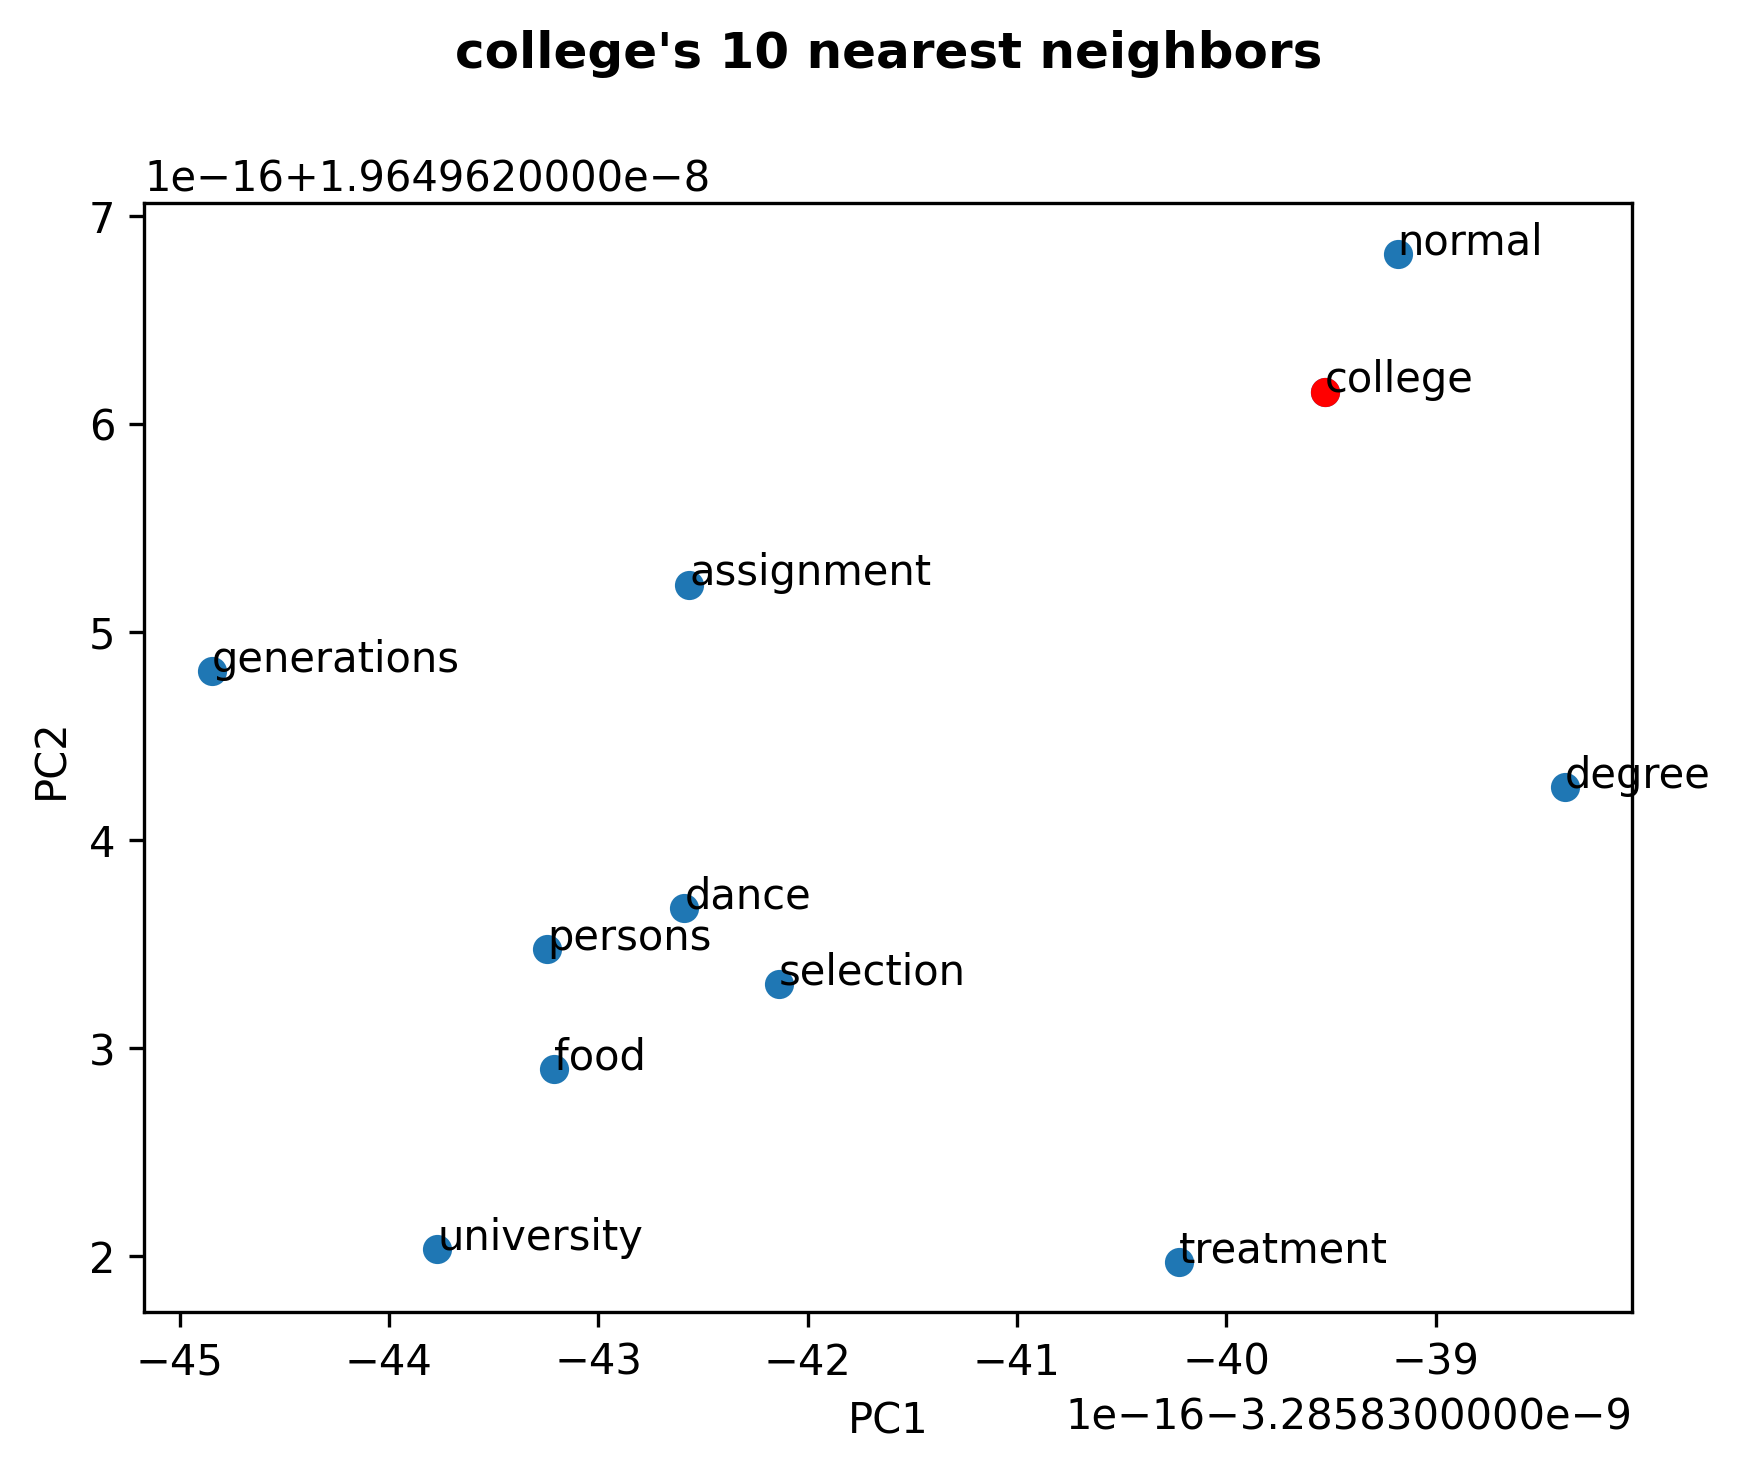
\includegraphics[width=0.8\textwidth]{../graphs/college_neighbors.png}
\end{center}
\caption{Top 10 nearest neighbors to "college" in the 100d vector space using cosine similarity}
\end{figure}

\begin{figure}[H]
\begin{center}
  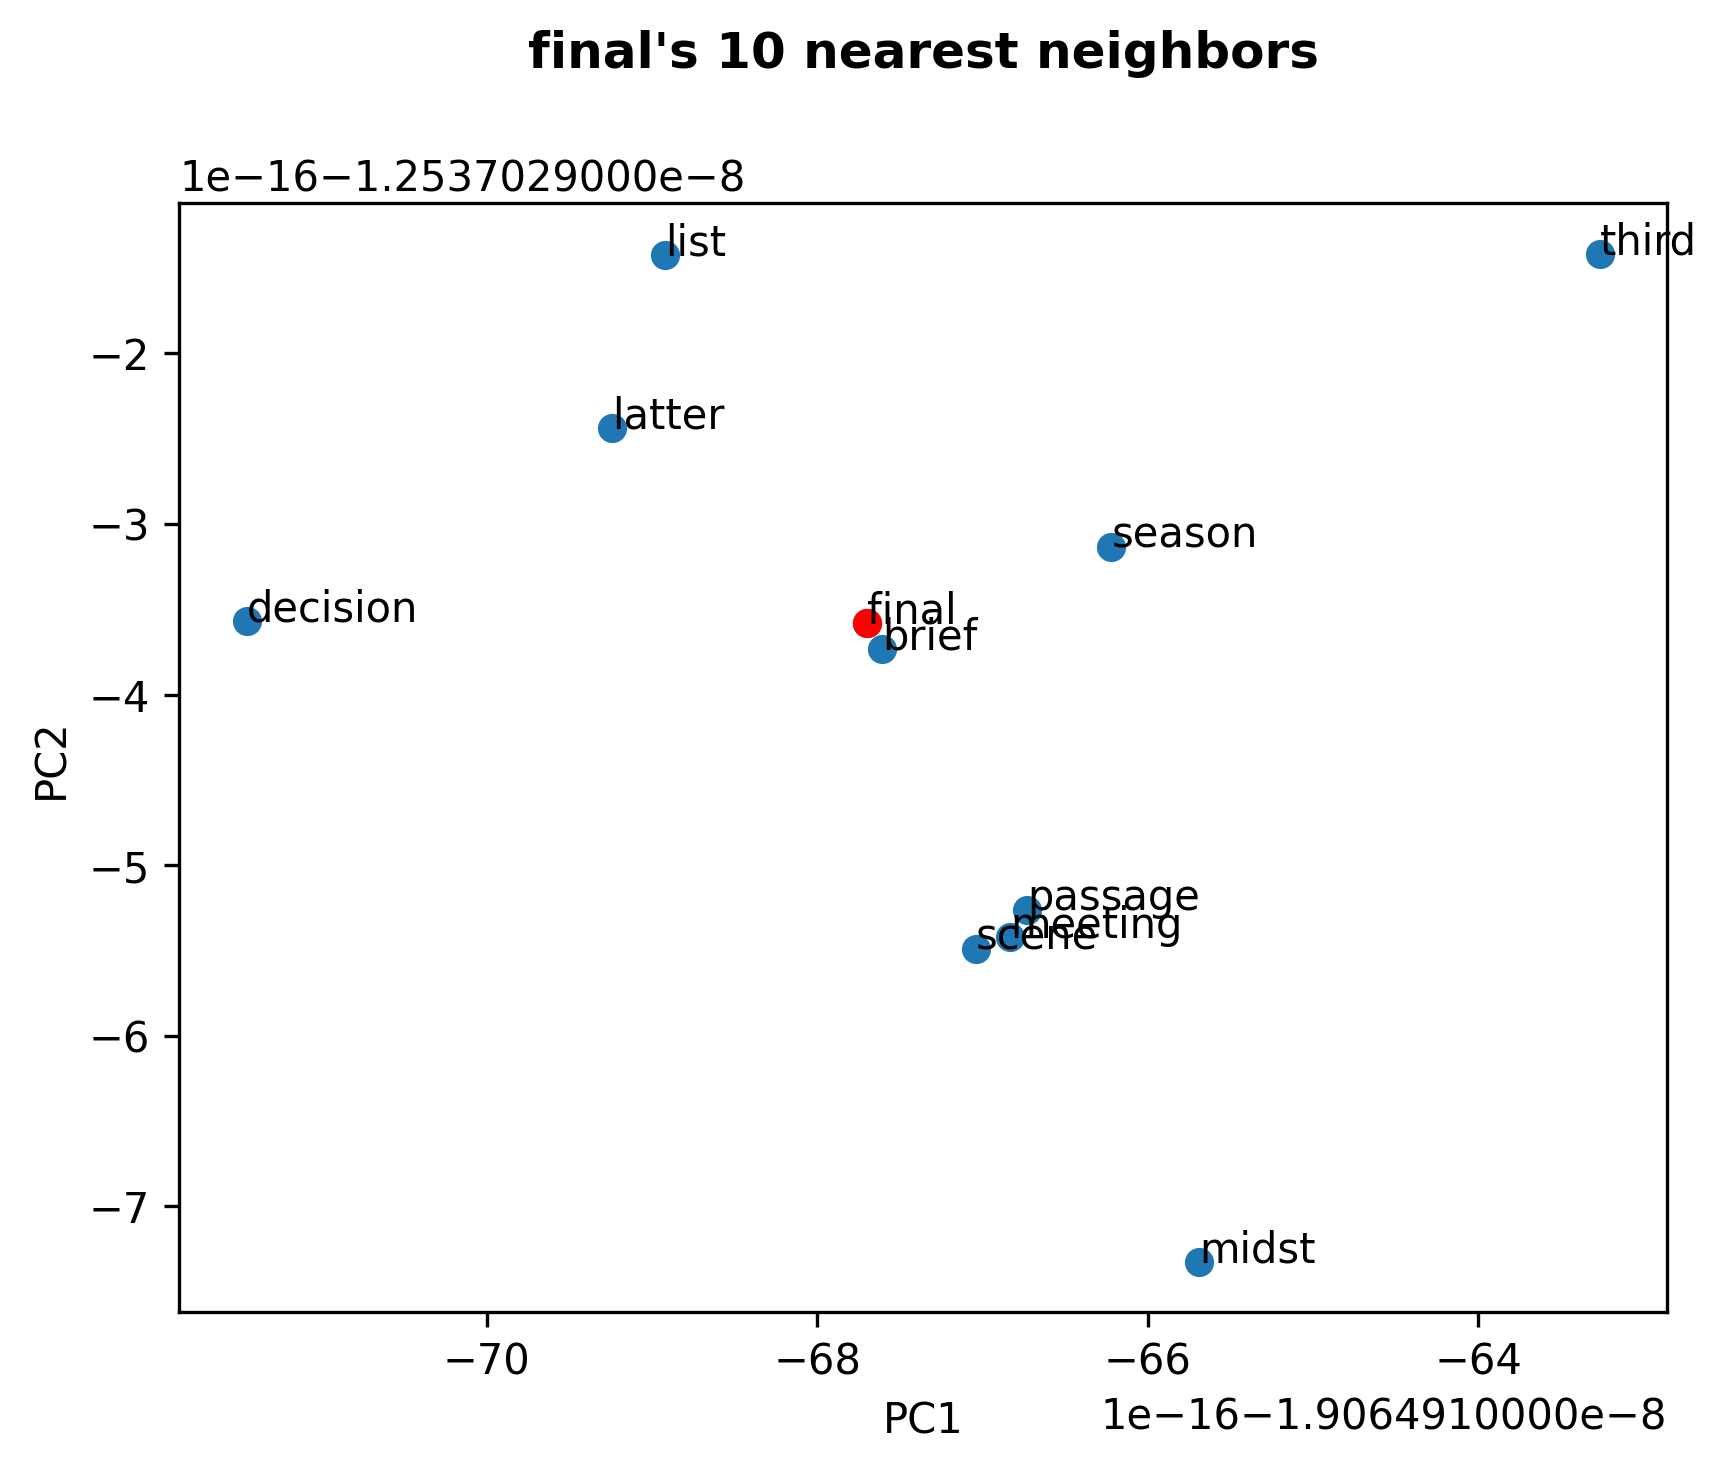
\includegraphics[width=0.8\textwidth]{../graphs/final_neighbors.png}
\end{center}
\caption{Top 10 nearest neighbors to "final" in the 2d vector space using PCA}
\end{figure}

\begin{figure}[H]
\begin{center}
  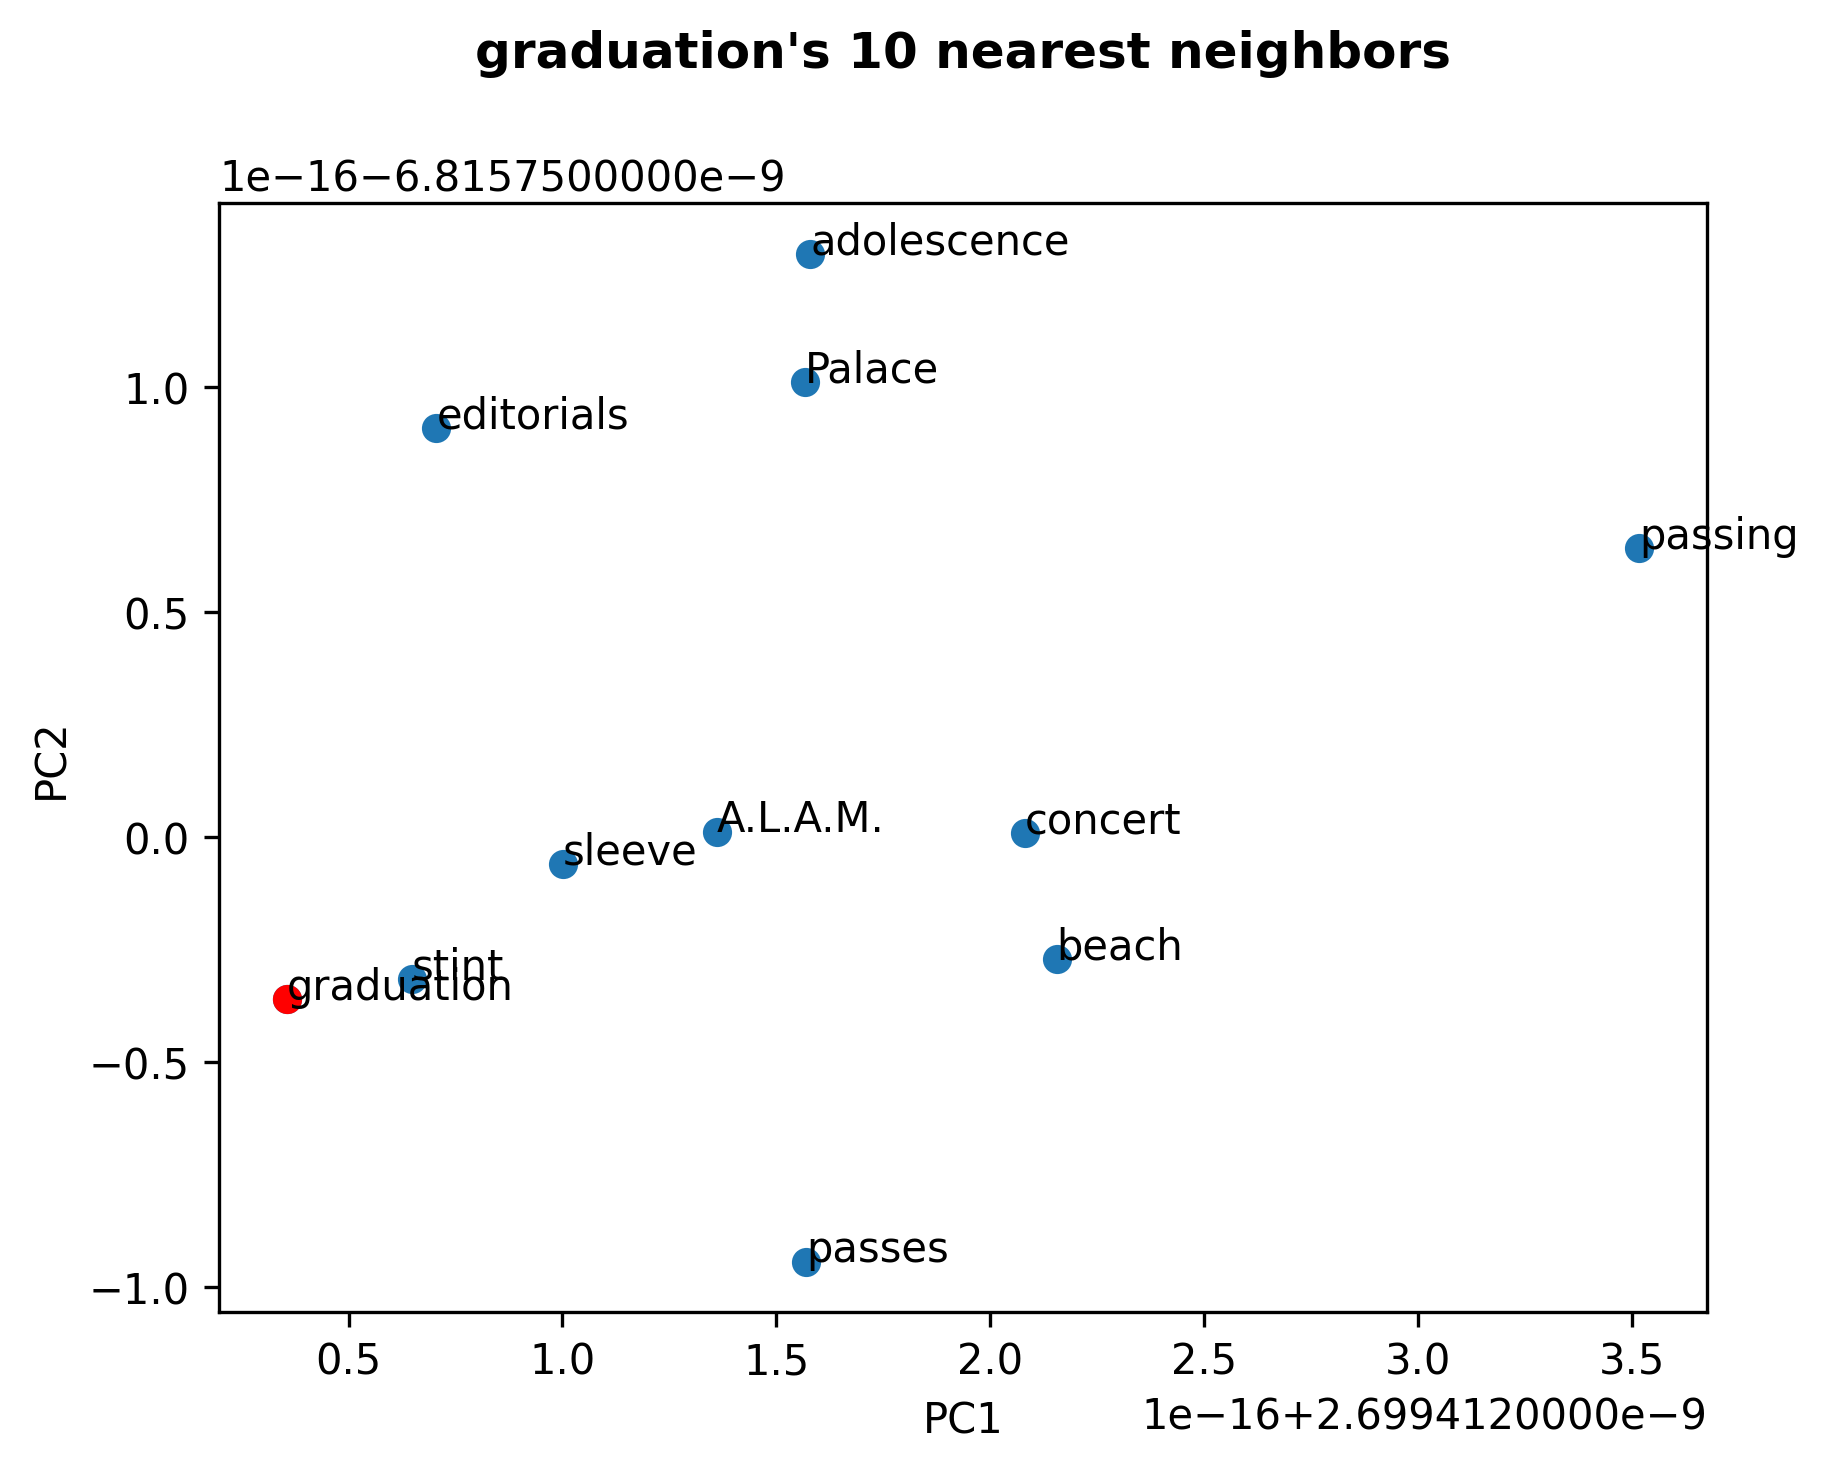
\includegraphics[width=0.8\textwidth]{../graphs/graduation_neighbors.png}
\end{center}
\caption{Top 10 nearest neighbors to "graduation" in the 2d vector space using PCA}
\end{figure}


\begin{figure}[H]
\begin{center}
  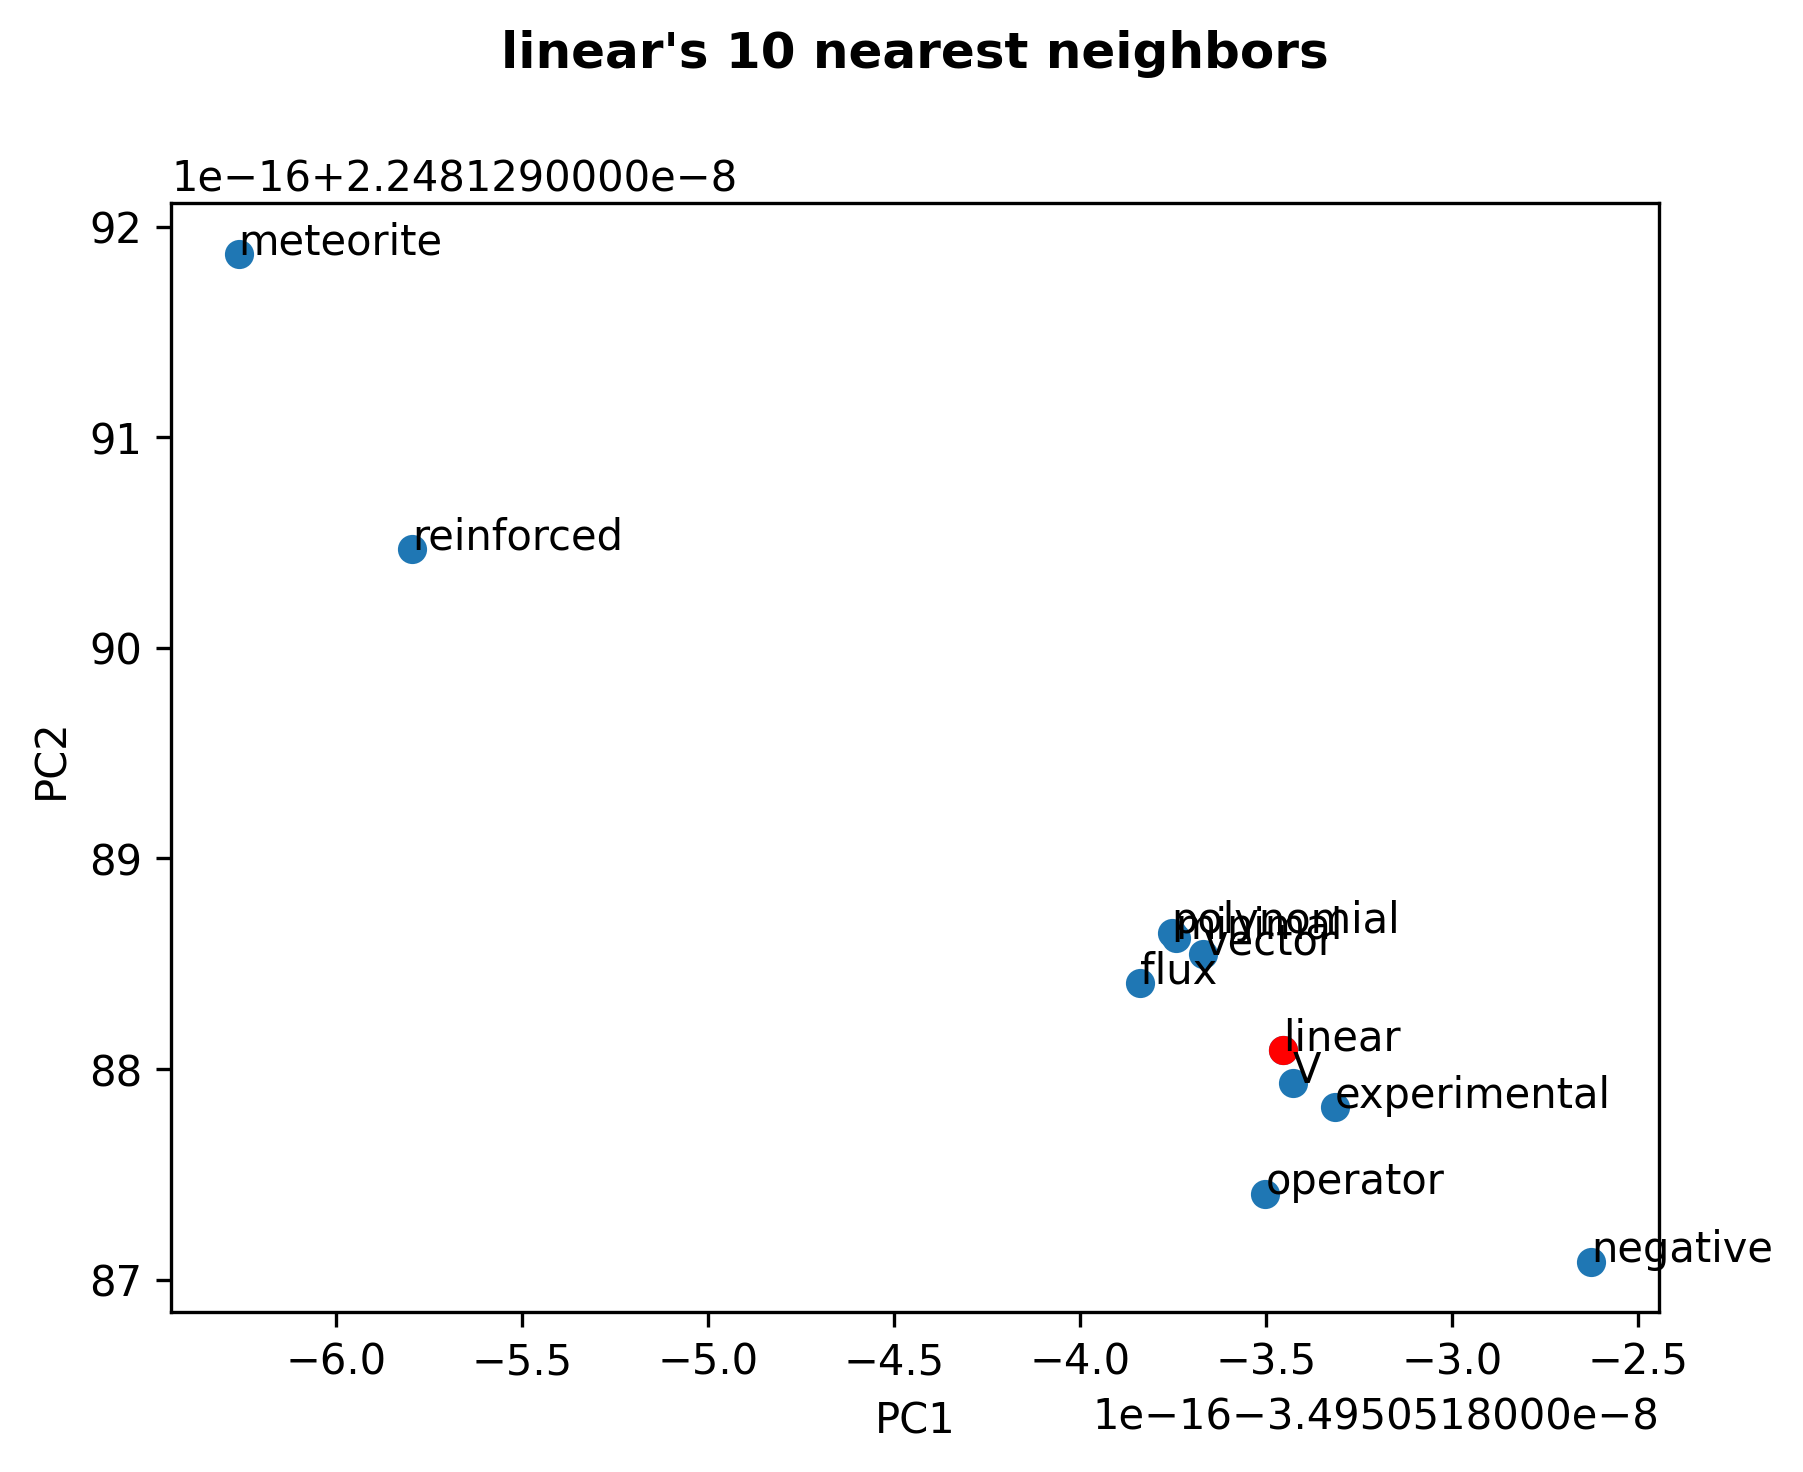
\includegraphics[width=0.8\textwidth]{../graphs/linear_neighbors.png}
\end{center}
\caption{Top 10 nearest neighbors to "linear" in the 2d vector space using PCA}
\end{figure}

\begin{figure}[H]
\begin{center}
  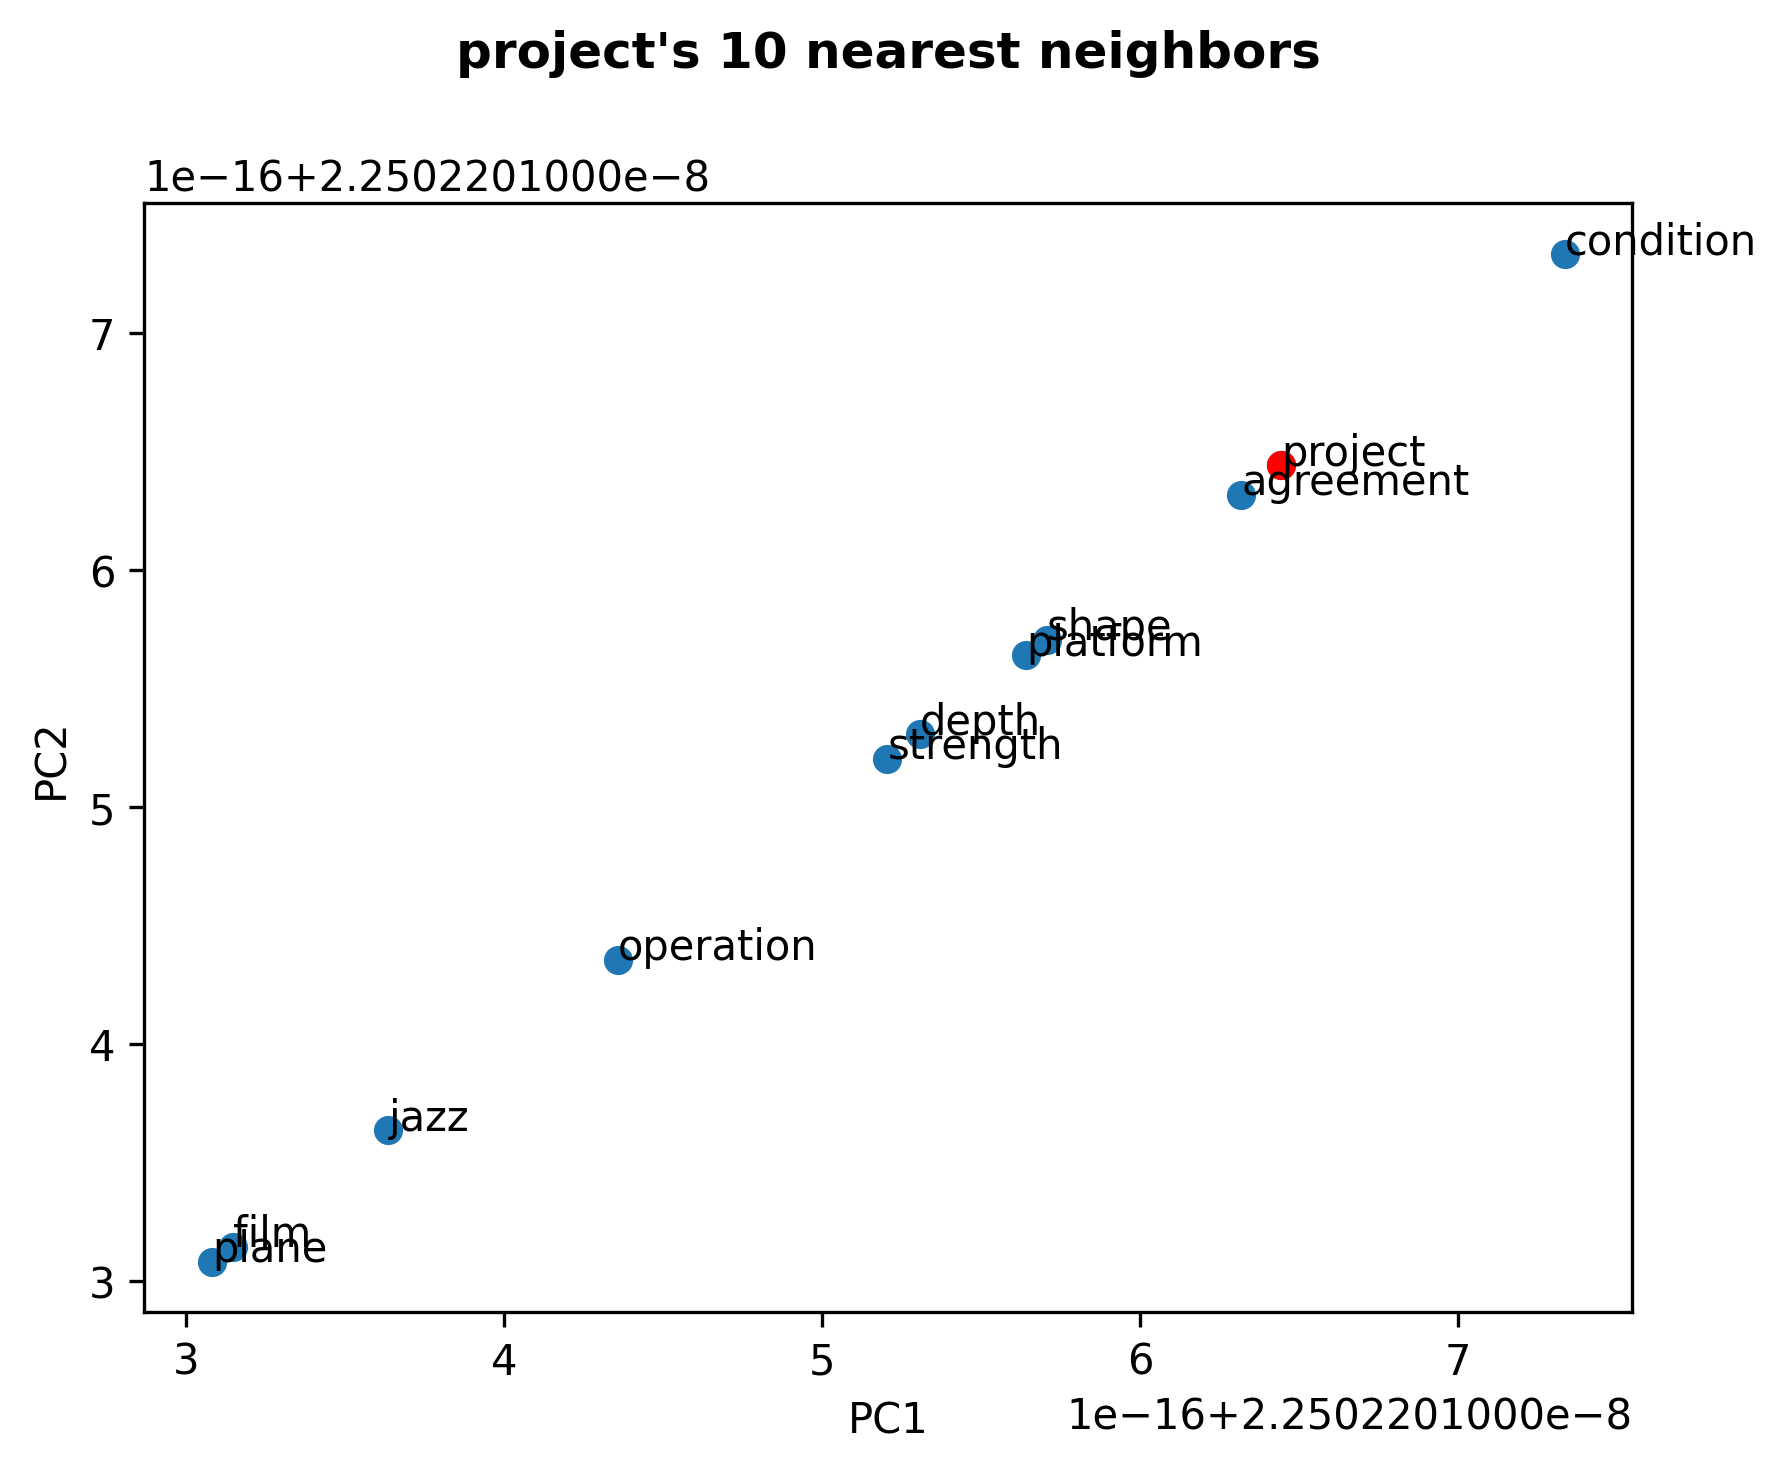
\includegraphics[width=0.8\textwidth]{../graphs/project_neighbors.png}
\end{center}
\caption{Top 10 nearest neighbors to "project" in the 2d vector space using PCA}
\end{figure}

\begin{figure}[H]
\begin{center}
  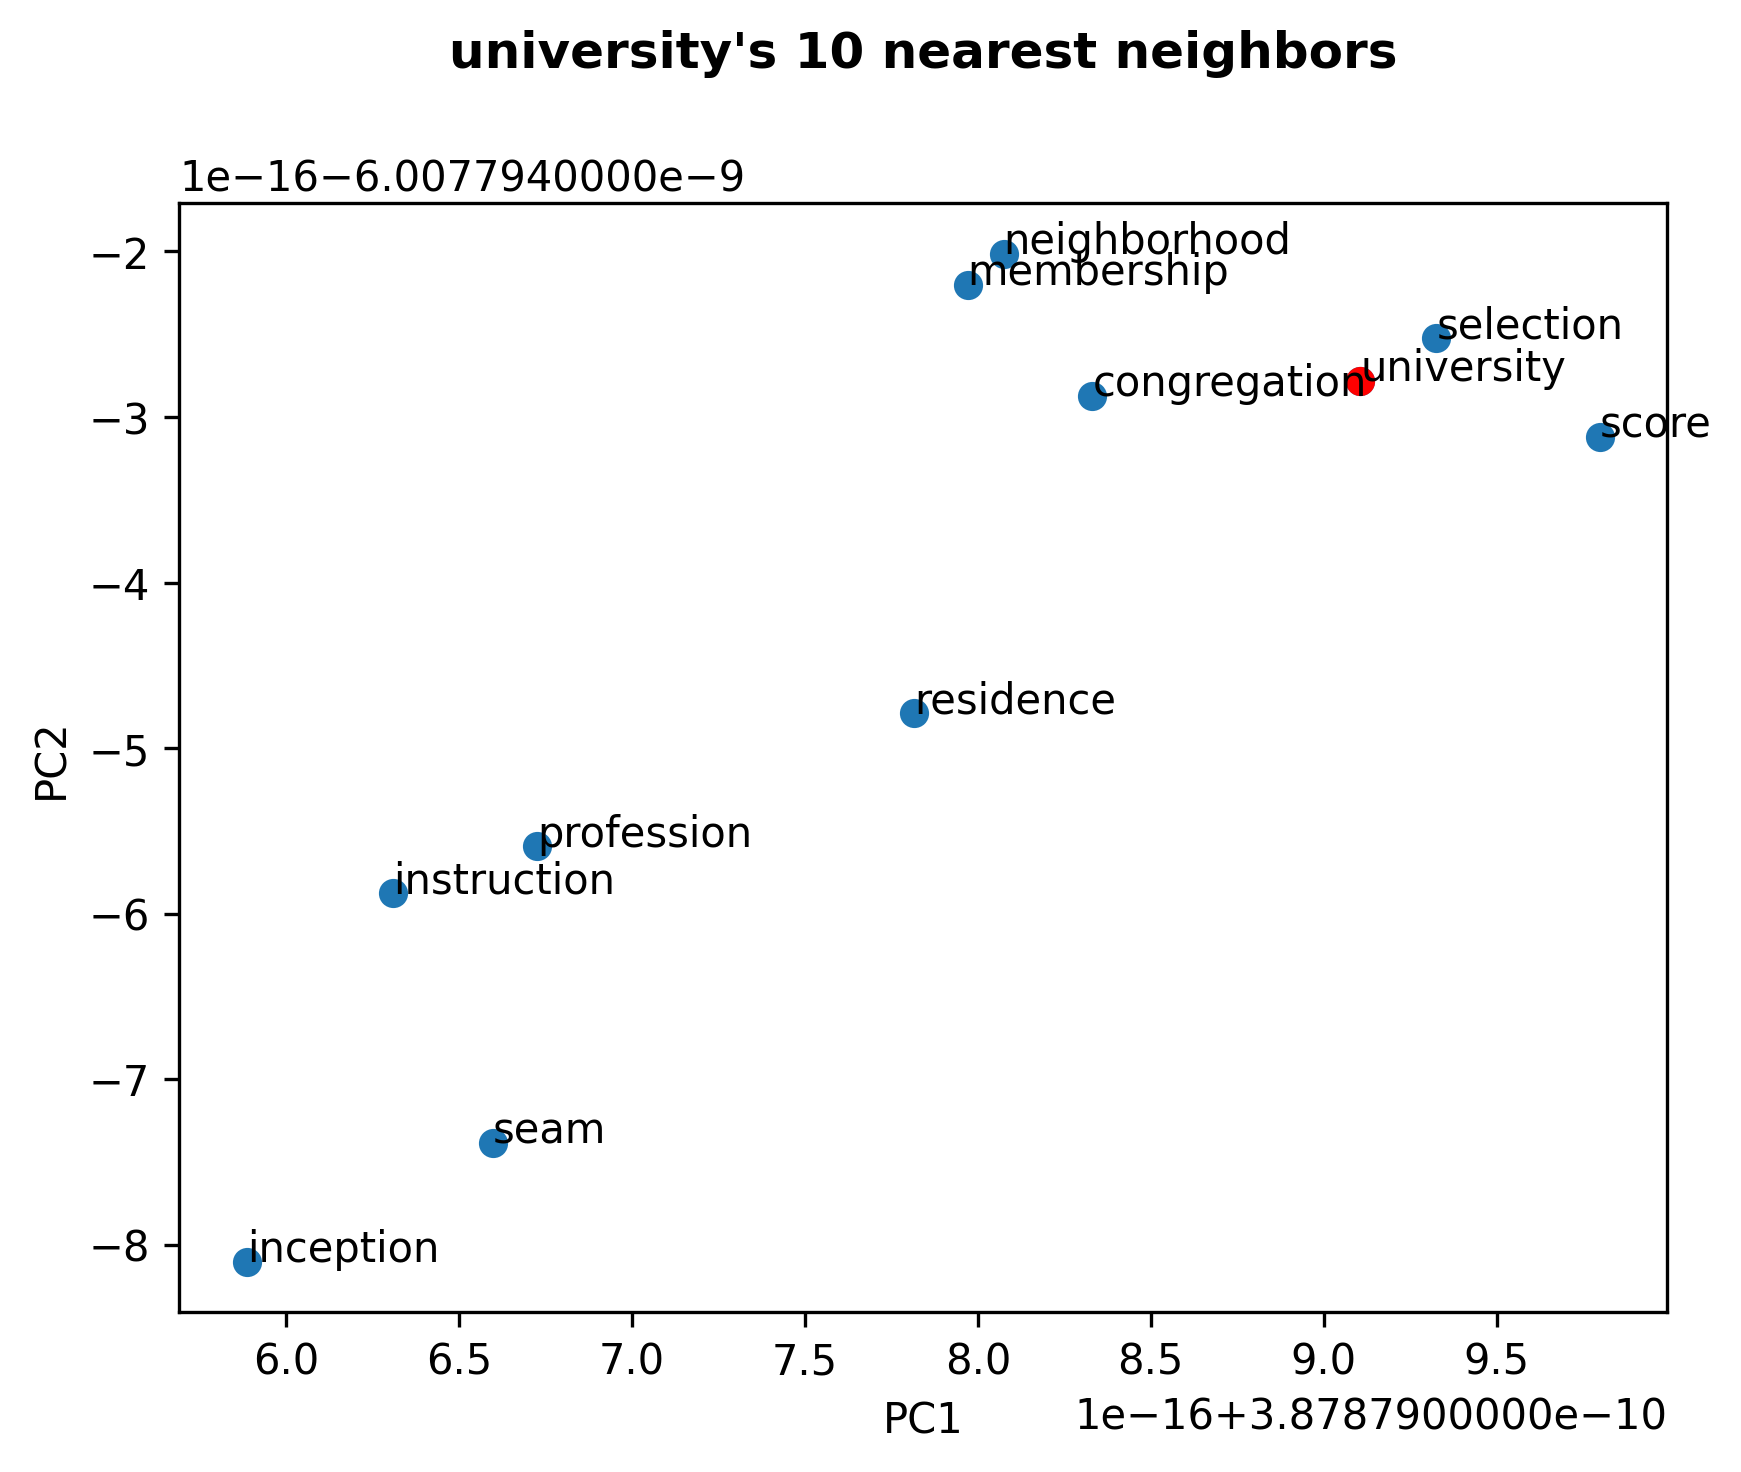
\includegraphics[width=0.8\textwidth]{../graphs/university_neighbors.png}
\end{center}
\caption{Top 10 nearest neighbors to "university" in the 2d vector space using PCA}
\end{figure}

\begin{figure}[H]
\begin{center}
  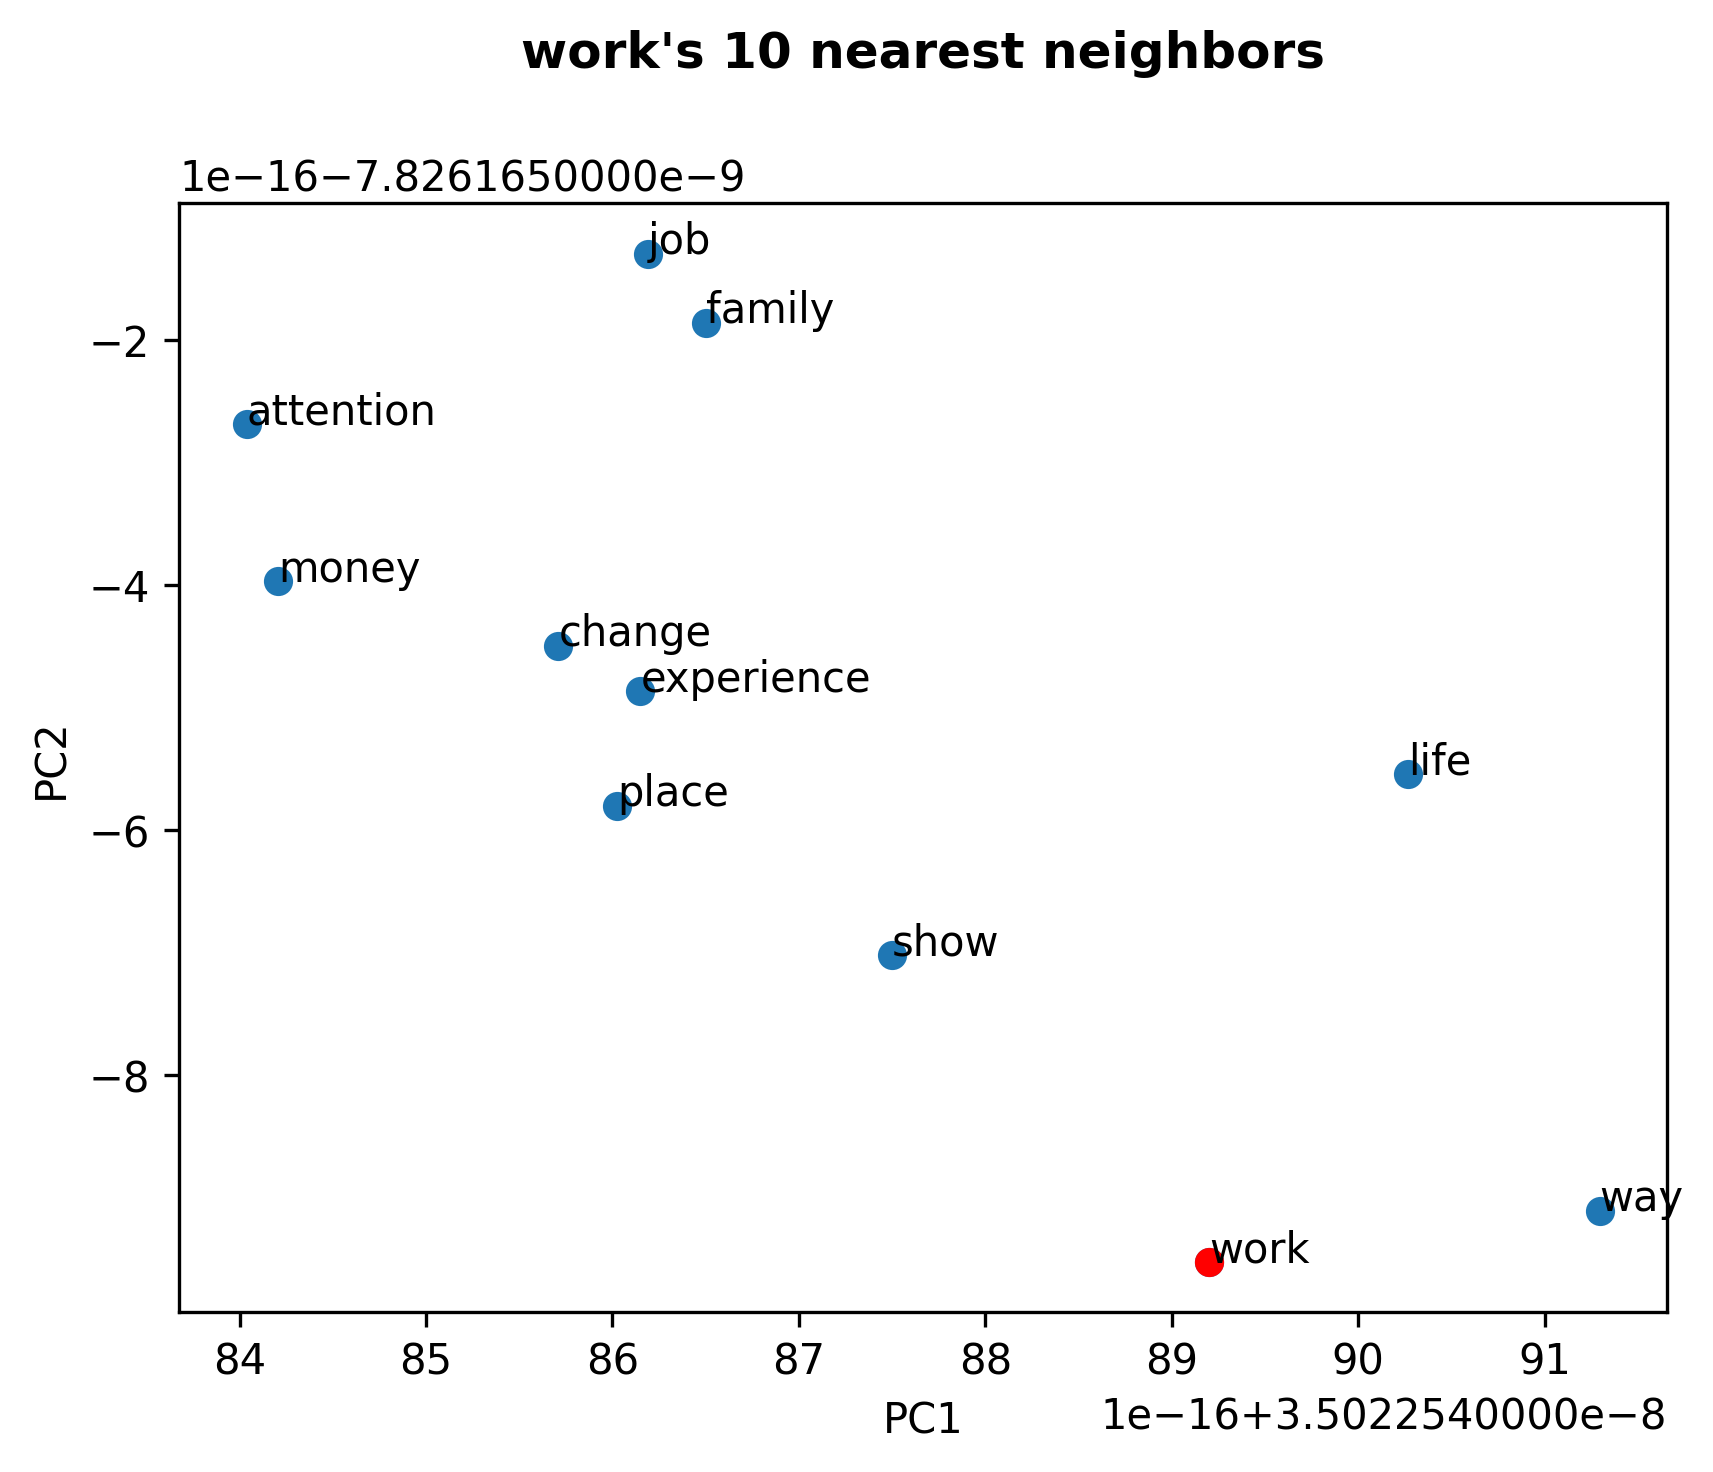
\includegraphics[width=0.8\textwidth]{../graphs/work_neighbors.png}
\end{center}
\caption{Top 10 nearest neighbors to "work" in the 2d vector space using PCA}
\end{figure}


\begin{thebibliography}{9}
\bibitem{word2vec}
WORD2VEC CITATION
\bibitem{browncorpus}
\bibitem{gensim}
\end{thebibliography}
\end{document}
